% !TEX TS-program = lualatex
% !TEX encoding = UTF-8 Unicode

\documentclass[professionalfonts]{beamer}
\usepackage{iftex,ifxetex}
\ifPDFTeX
  \usepackage[utf8]{inputenc}
  \usepackage[T1]{fontenc}
  \usepackage{lmodern}
\else
  \ifluatex
    \usepackage{unicode-math} 
    \defaultfontfeatures{Ligatures=TeX}
    % \setmathfont{Latin Modern Math}
    \setsansfont{CMU Sans Serif}
    % \setsansfont{Linux Biolinum O}
  \fi
\fi

\mode<presentation>
{
  \usetheme{Madrid} % or try Darmstadt, Madrid, Warsaw, ...
  % or ...
  \setbeamertemplate{bibliography item}{}
  \setbeamercovered{transparent}
  % or whatever (possibly just delete it)
}

\usepackage{fontspec}
\usepackage[english]{babel}
% or whatever
\usepackage{csquotes}
\usepackage[backend=biber,
        style=unified,
        maxcitenames=3,
        maxbibnames=99,
        natbib,
        url=false]{biblatex}
% \addbibresource{Dissertation.bib}
\setmainfont{Libertinus Sans} % Main font
% \setsansfont{libertinus sansserif} % Sans serif font
% \setmonofont{CMU Typewriter Text}
\renewcommand{\ttdefault}{cmtt}

% \usepackage[colorlinks,allcolors={black},urlcolor={blue}]{hyperref} %allows for hyperlinks and pdf bookmarks 
\usepackage{graphicx}	%Inserting graphics, pictures, images 		
\usepackage{multicol} %Multicolumn text
\usepackage{multirow} %Useful for combining cells in tablesbrew 
% \usepackage{booktabs} %Enhanced tables
% \usepackage{underscore} %Allows for underscores in text mode
% \usepackage[colorlinks,allcolors={black},urlcolor={blue}]{hyperref} %allows for hyperlinks and pdf bookmarks
\usepackage{url} %allows for urls
\def\UrlBreaks{\do\/\do-} %allows for urls to be broken up
% \usepackage[normalem]{ulem} %strike out text. Handy for syntax
% \usepackage{tcolorbox}
% \usepackage{datetime2}
\usepackage{caption}
\usepackage{subcaption}
\usepackage{langsci-gb4e} % Language Science Press' modification of gb4e
\usepackage{tikz} % Drawing Hasse diagrams
\usetikzlibrary{decorations.pathreplacing}
\usepackage{leipzig} %	Offers support for Leipzig Glossing Rules
% \usepackage{animate} % For creating animations in PDF slides
\usepackage{annotate-equations}

% Hyperlink settings
\hypersetup{
    colorlinks,
    urlcolor=blue,        % Color for URLs
    linkcolor=white        % Color for internal links
}

\title[LING 450/550] % (optional, use only with long paper titles)
{Introduction to Linguistic Phonetics}

\subtitle{Sounds and Waves}

\author[Brinkerhoff] % (optional, use only with lots of authors)
{Mykel Loren Brinkerhoff}
% - Give the names in the same order as the appear in the paper.
% - Use the \inst{?} command only if the authors have different
%   affiliation.

\institute[UW] % (optional, but mostly needed)
{University of Washington}
% - Use the \inst command only if there are several affiliations.

\date[2025-10-07] % (optional, should be abbreviation of conference name)
{October 7, 2025}

% If you have a file called "university-logo-filename.xxx", where xxx
% is a graphic format that can be processed by latex or pdflatex,
% resp., then you can add a logo as follows:

% \pgfdeclareimage[height=0.5cm]{university-logo}{university-logo-filename}
% \logo{\pgfuseimage{university-logo}}



% Delete this, if you do not want the table of contents to pop up at
% the beginning of each subsection:
% \AtBeginSubsection[]
% {
%   \begin{frame}<beamer>{Outline}
%     \tableofcontents[currentsection,currentsubsection]
%   \end{frame}
% }


% If you wish to uncover everything in a step-wise fashion, uncomment
% the following command: 

%\beamerdefaultoverlayspecification{<+->}


\begin{document}

\begin{frame}
    \titlepage
\end{frame}

%-----------------------------------------------------------
\section{Introduction}
%-----------------------------------------------------------

% \begin{frame}{Which medieval cat are you?}
    
%     \begin{center}
%         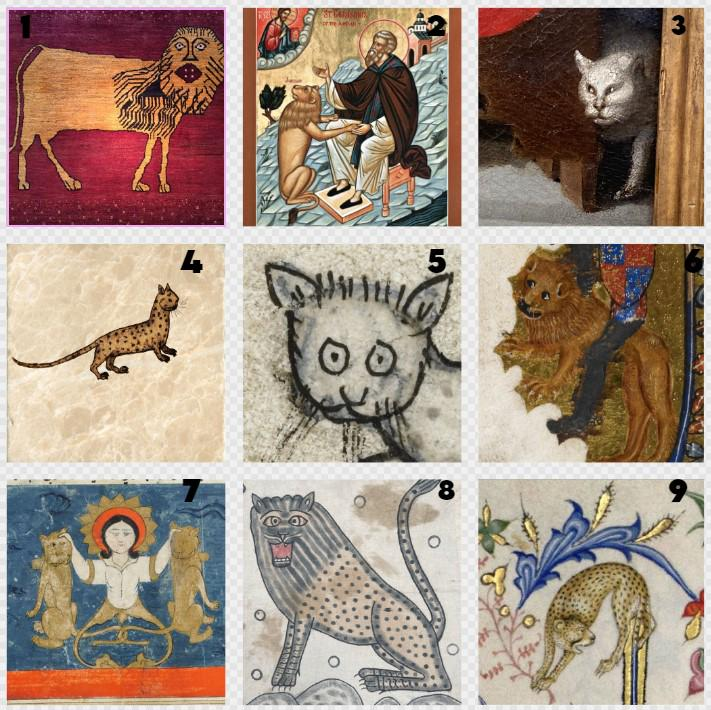
\includegraphics[width = .5\linewidth]{figs/MedievalCatIcebreaker.jpeg}
%         \url{https://pollev.com/mykellorenbrinkerhoff821} or text/SMS mykellorenbrinkerhoff821 to 22333
%     \end{center}
% \end{frame}

\begin{frame}{Recap and Reflection}
    \begin{block}{Reflection}
        \begin{itemize}
            \item Spend $\thicksim$3 minutes reviewing your notes from last lecture, homeworks, exit tickets, etc.
            \item Look for questions you have or clarifications you would like. 
        \end{itemize}
    \end{block}
\end{frame}

%-----------------------------------------------------------
\section{Sound Waves}
%-----------------------------------------------------------

% \begin{frame}{Sound and waves}
    % \begin{center}
    %     \animategraphics[
    %         loop,           % Loop the animation
    %         controls,       % Show play/pause controls
    %         width=0.6\textwidth,
    %         autoplay        % Start automatically
    %     ]{12}{figs/monopole_animate/frame_}{001}{031}
    % \end{center}
% \end{frame}

\begin{frame}{What is sound?}
    \begin{itemize}
        \item The basic definition = a pressure wave that moves through some medium (like air, water, etc.)
        \item It is a vibration of the particles in that medium, and it propagates, or moves, through the medium 
    \end{itemize}
\end{frame}

\begin{frame}{Acoustic waves}
    \begin{itemize}
        \item Acoustic waves are typically generated by compression of particles, which then expand back to their original position
        \item This \textbf{compression} and expansion (more technically called \textbf{rarefaction}) expands and affects nearby particles, spreading in a wave-like pattern
        \begin{itemize}
            \item Important: the particles themselves move in a relatively restricted area, the waves travel much further!
            \item It can be analogized to be spring-like or slinky-like (see images)
        \end{itemize}
        \item Sound waves in gasses and liquids travel as \textbf{longitudinal} waves
        \begin{itemize}
            \item \href{https://www.acs.psu.edu/drussell/demos/waves/wavemotion.html}{Examples} of wave types from Daniel Russell
            \item \href{https://youtu.be/_WsAQo8uMhY?si=RpFxY4ZQzH9kzfql&t=865}{The Magic Schoolbus - Inside the Haunted House (14:25–17:50)}
        \end{itemize}
    \end{itemize}
\end{frame}

\begin{frame}{Wave propagation}
    \begin{itemize}
        \item Sound waves “propagate” or move away from the source in all directions, unless obstructed or modified by changes in the medium
        \item The speed of propagation of sound in air depends on the temperature and humidity
        \begin{itemize}
            \item In our atmosphere, near sea level it is $\approx$ 34,300cm/s (343m/s, 767mph\footnote{For us non-SI crazies.})
            \item In water, it's 148,000cm/s (1480m/s, 3310mph)
            \item The vocal tract is fairly warm and humid, and the speed of sound is $\approx $35,000cm/s (350m/s, or 783mph)
            \begin{itemize}
                \item This is what we will be using for the speed of sound. 
            \end{itemize}
            \item If sound is traveling through a different medium, that \href{https://youtu.be/d-XbjFn3aqE?si=3AE-7EA5ck7BWhJa}{differs in density}, it might be faster or slower 
        \end{itemize}
    \end{itemize}
\end{frame}

\begin{frame}{Wave propagation}
    \begin{center}
        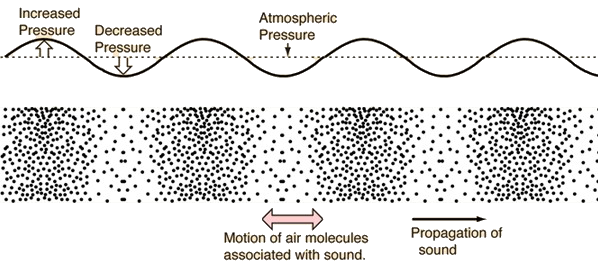
\includegraphics[width = 0.75\textwidth]{figs/OscillogramPressure.png}
    \end{center}
    \begin{itemize}
        \item Top part is the \textbf{waveform} (fancier term: \textbf{oscillogram}) and graphically represents sound waves
        \begin{itemize}
            \item It shows changes from \textbf{atmospheric equilibrium} 
            \item We typically assign zero to atmospheric equilibrium and refer to relative changes from it 
            \item Thus it is commonly called the \textbf{zero}, or \textbf{zero line}
        \end{itemize}
        \item Bottom shows the compression and rarefaction of the particles
    \end{itemize}
\end{frame}

%-----------------------------------------------------------
\section*{Periodicity and Aperiodicity}
%-----------------------------------------------------------

\begin{frame}{Two types of waves}
    \begin{itemize}
        \item \textbf{Periodic}
        \begin{itemize}
            \item Wave with a regularly repeating pattern 
            \item Examples: Bowed string instrument, voiced sounds 
        \end{itemize}
        \item \textbf{Aperiodic}
        \begin{itemize}
            \item No discernible repeating pattern in the wave 
            \item Can be continuously produced, still without a repeating pattern (e.g. white noise, pink noise, fricatives) 
            \item A single burst of aperiodic sound is called a transient (e.g. a clap, drum hit, stop burst)
        \end{itemize}
    \end{itemize}
\end{frame}

%-----------------------------------------------------------
\subsection*{Periodic Waves}
%-----------------------------------------------------------

\begin{frame}{Periodic Waves}
    \begin{itemize}
        \item \textbf{Frequency} 
        \begin{itemize}
            \item The rate at which a portion of a wave (a period) repeats in a given time unit 
            \item Unit of measure: periods (cycles) per second, called \textbf{Hertz} (\textbf{Hz})
        \end{itemize}
        \item \textbf{Wavelength} ($\lambda$)
        \begin{itemize}
            \item Distance (in meters) from one period to the next
        \end{itemize}
        \item \textbf{Amplitude}
        \begin{itemize}
            \item Magnitude of the oscillation, measured in Pascals (absolute), or Decibels (relative)
        \end{itemize}
    \end{itemize}
\end{frame}

\begin{frame}{Frequency}
    \begin{multicols}{2}
        \begin{itemize}
            \item The rate at which a cycle/period repeats
            \item More frequent repetitions are perceived as having higher pitch than less frequent ones
            \item Western (equal temperament) \href{https://mixbutton.com/music-tools/frequency-and-pitch/music-note-to-frequency-chart}{musical tuning and frequency}
        \end{itemize}

        \columnbreak

        \begin{center}
            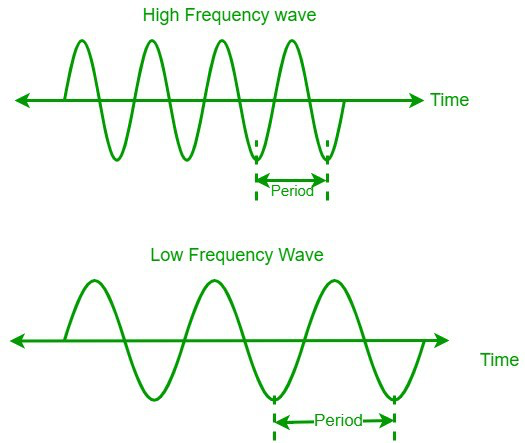
\includegraphics[width = \linewidth]{figs/Frequency.png}
        \end{center}
    \end{multicols}
\end{frame}

\begin{frame}{Wavelength ($\lambda$)}
    \begin{multicols}{2}
        \begin{center}
            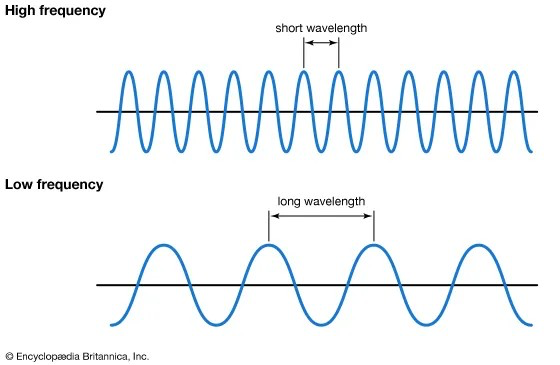
\includegraphics[width = \linewidth]{figs/Wavelength.png}
        \end{center}
        \vspace{3em}
        \begin{equation*}
            \tikzmarknode{lambda}{\lambda} = \frac{\tikzmarknode{c}{c}}{\tikzmarknode{f}{f}}
        \end{equation*}
        \annotate[yshift=1em]{left}{lambda}{wavelength}
        \annotate[yshift=1em]{right}{c}{speed of sound (m/s)}
        \annotate[yshift=-0.5em]{below, label below}{f}{frequency (Hz)}
        \columnbreak
        \begin{itemize}
            \item The distance from one period to another, using the same part of the wave
            \begin{itemize}
                \item e.g., peak–to–peak, trough–to–trough, positive zero crossing to positive zero crossing
            \end{itemize}
            \item Represented as the Greek letter lambda ($\lambda$)
            \item Inversely related to frequency (longer wavelength → lower frequency)
        \end{itemize}
    \end{multicols}
\end{frame}

\begin{frame}{Amplitude}
    \begin{multicols}{2}
        \begin{itemize}
            \item Amplitude is how far the particles move away from equilibrium, show on a waveform by how high the peaks and low the troughs are from the zero line
            \item In simple terms, we hear this as loudness: the greater the amplitude, the louder the sound
            \item We'll go more in-depth later when we talk about audition
        \end{itemize}
        \columnbreak
        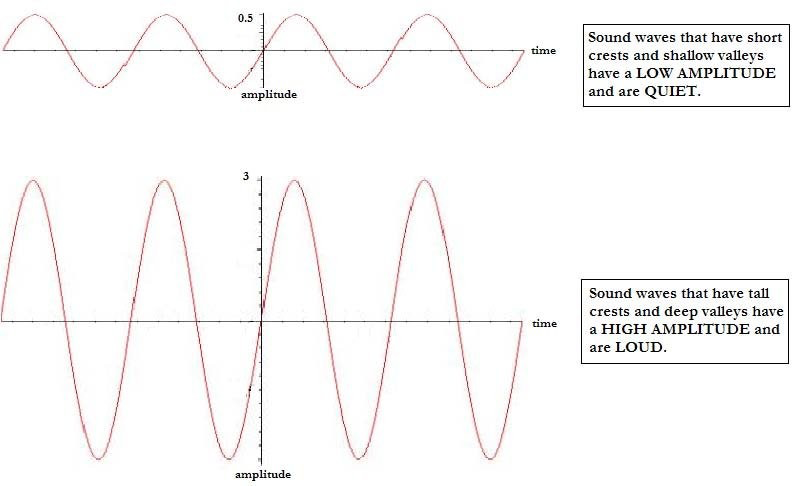
\includegraphics[width = \linewidth]{figs/Amplitude.png}
    \end{multicols}
\end{frame}

%-----------------------------------------------------------
\section*{Aperiodic Waves}
%-----------------------------------------------------------

\begin{frame}{Aperiodic waves}
    \begin{itemize}
        \item No repeating pattern
        \item No consistent wavelength
        \item Overall amplitude might be consistently within a range, but not on small scale
        \item Related to turbulent airflow
        \item \href{https://en.wikipedia.org/wiki/White_noise}{white noise} and \href{https://en.wikipedia.org/wiki/Pink_noise}{pink noise} are two mathematically defined types
    \end{itemize}
\end{frame}

%-----------------------------------------------------------
\section*{Break}
%-----------------------------------------------------------

\begin{frame}{Break Time!}
    \begin{center}
        \Huge 10 minute break \\ (stretch, grab a drink, etc.)
    \end{center}
\end{frame}

%-----------------------------------------------------------
\section*{Complex Waves and spectra}
%-----------------------------------------------------------

\begin{frame}{Complex waves and spectra}
    \begin{center}
        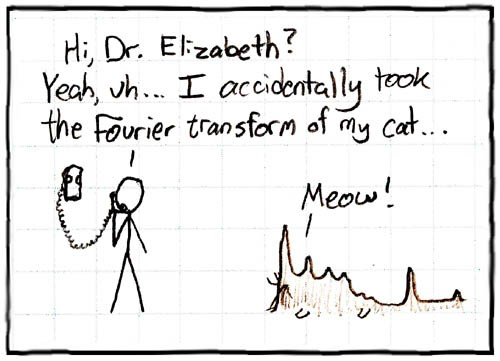
\includegraphics[width = 0.75\linewidth]{figs/FourierCats.jpg}    
    \end{center}
    
    {\footnotesize Image copyright Randall Munroe, XKCD comics}
\end{frame}

\begin{frame}{Simple period waves}
    \begin{itemize}
        \item A very specific type of wave defined by the \textbf{sine} trigonometric function
        \item Important because it forms the building block for more complex sounds
        \item \href{https://www.acs.psu.edu/drussell/Demos/complex/complex.html}{It is geometrically related to a circle}
    \end{itemize}
\end{frame}

\begin{frame}{Sine and Cosine waves}
    \begin{itemize}
        \item Sine and Cosine waves are closely related
        \item The difference between the two can be described as a \textbf{phase} difference
    \end{itemize}
\end{frame}

\begin{frame}{Superposition of waves}
    \begin{multicols}{2}
        \begin{itemize}
        \item When waves interact, the result is constructive or destructive interference
        \begin{itemize}
            \item Constructive = additive 
            \item Destructive = subtractive
        \end{itemize}
    \item Adding simple waves together results in a \textbf{complex wave}
    \end{itemize}

    \columnbreak

    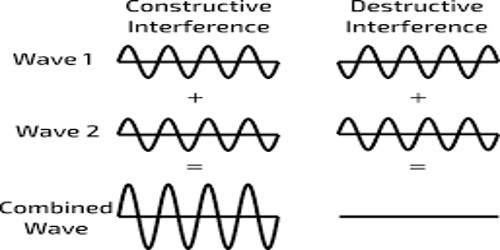
\includegraphics[width = \linewidth]{figs/ConstructiveDestructive.png}
    \end{multicols}
\end{frame}

\begin{frame}{“Adding” waves}
    \begin{multicols}{2}
        \begin{itemize}
            \item The phasing of waves matters to how they will combine
            \item At left, the waves are in phase (top), 90° out of phase, and 180° out of phase (bottom)
            \item If we add these waves, we get constructive and destructive interference
        \end{itemize}

        \columnbreak

        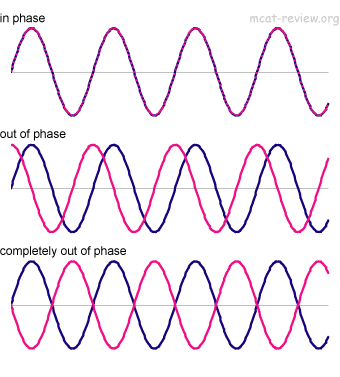
\includegraphics[width = \linewidth]{figs/Phasing.png}
    \end{multicols}
\end{frame}

\begin{frame}{Illustration of Constructive and Desctructive Interference}
    \begin{center}
        \href{https://www.acs.psu.edu/drussell/Demos/superposition/interference.gif}{Interference Illustration}
    \end{center}
\end{frame}

\begin{frame}{Superposition of waves}
    \begin{multicols}{2}
        \begin{itemize}
            \item So far all the waves we’ve discussed in this section are the same frequency and amplitude
            \item Things get slightly more complicated for waves of different frequencies and amplitudes
        \end{itemize}
        \columnbreak
        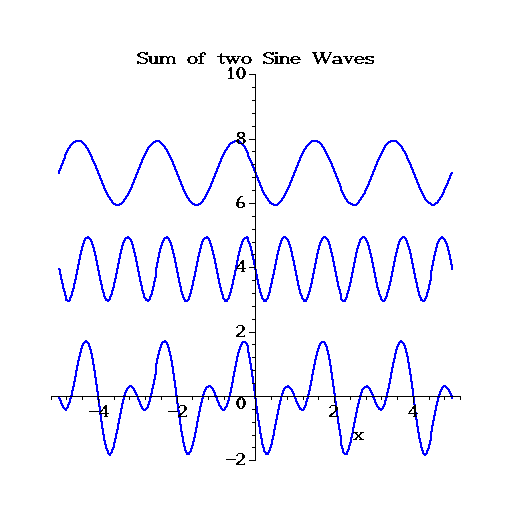
\includegraphics[width = \linewidth]{figs/AddingSines.png}
    \end{multicols}
\end{frame}

\begin{frame}{Complex waves}
    \begin{multicols}{2}
        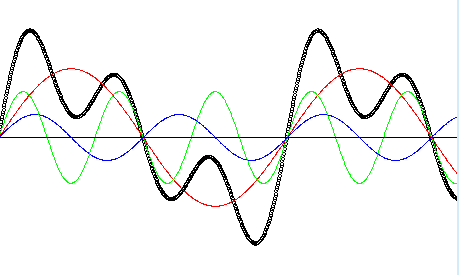
\includegraphics[width = \linewidth]{figs/Complex.png}

        \columnbreak

        \begin{itemize}
            \item The simple waves we’ve been discussing don’t exist in nature on their own
            \item The sound waves all around us are \textbf{complex waves} made up of many simple waves
            \item You can generate some using \href{https://www.falstad.com/fourier/}{this applet}
        \end{itemize}
    \end{multicols}
\end{frame}

\begin{frame}{Components of complex waves}
    \begin{itemize}
        \item Since waves combine into more complex ones predictably, we can take complex ones and break them down into their simple \textbf{components}
        \item This is actually a bit complicated, but modern computing makes it easy
        \begin{itemize}
            \item Praat has this built in.
        \end{itemize}
        \item It’s called \textbf{Fourier Analysis}
    \end{itemize}
\end{frame}

\begin{frame}
    \frametitle{Fourier Analysis}

    \begin{multicols}{2}
        \begin{itemize}
            \item This process takes a complex wave and breaks it down into its component waves
            \item In terms of periodic waves, we get the frequency and amplitude of those waves
        \end{itemize}

        \columnbreak

        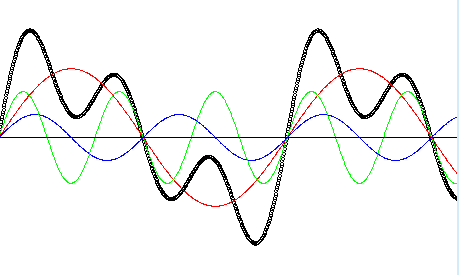
\includegraphics[width = \linewidth]{figs/Complex.png}
    \end{multicols}
\end{frame}

\begin{frame}
    \frametitle{Visualizing component waves}
    \begin{multicols}{2}
        \begin{itemize}
            \item Fourier analysis Waveform produces a spectrum
            \item A spectrum shows a snapshot of a sound
            \item This snapshot shows the amplitude and frequency of component waves
        \end{itemize}
        
        \columnbreak

        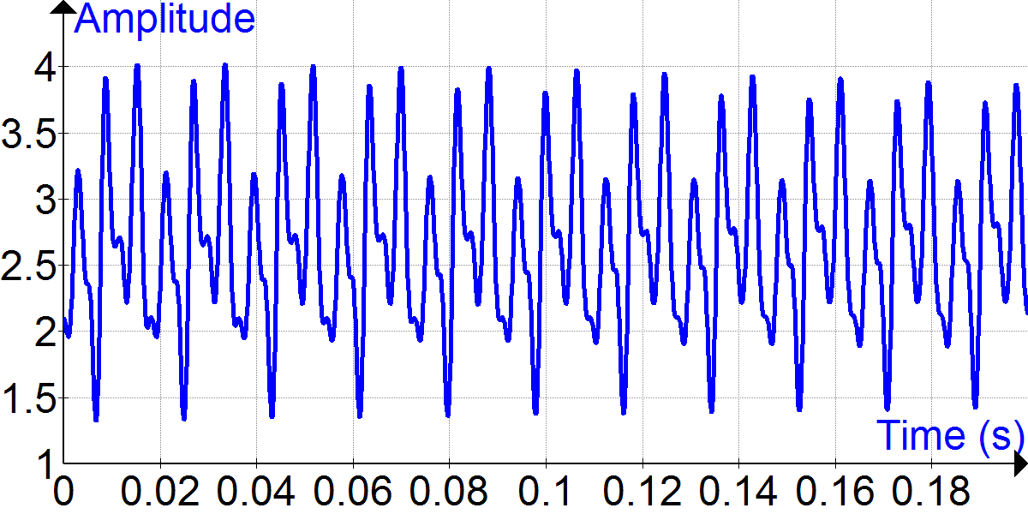
\includegraphics[width = \linewidth]{figs/ComplexWaves.png}
        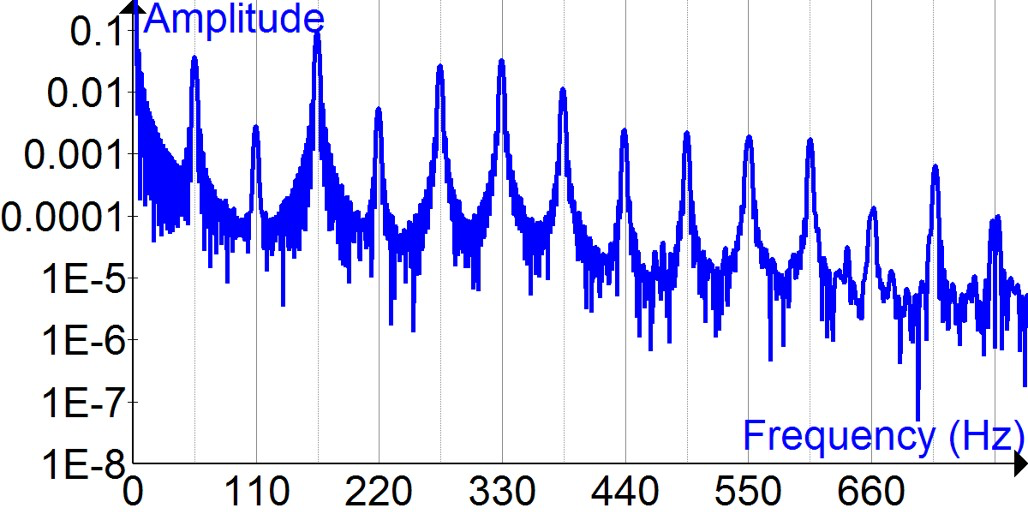
\includegraphics[width = \linewidth]{figs/Fourier-ComplexWaves.png}
    \end{multicols}
\end{frame}

\begin{frame}{Spectrum (pl. spectra)}
    \begin{multicols}{2}
        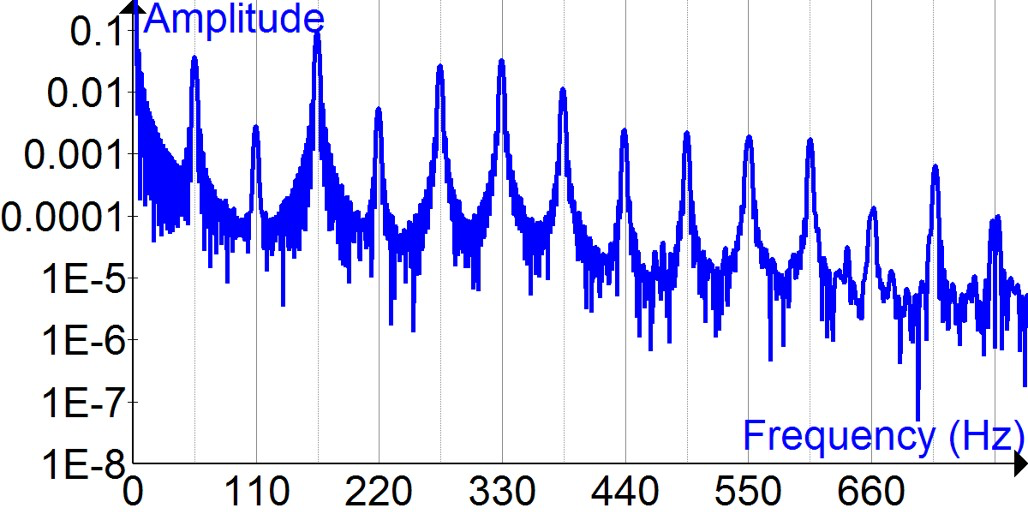
\includegraphics[width = \linewidth]{figs/Fourier-ComplexWaves.png}
        \columnbreak

        \begin{itemize}
            \item X-axis shows frequency
            \item Y-axis shows amplitude
            \item This is a mathematical estimation, so there’s some “fuzziness”, especially in the lower amplitude
        \end{itemize}
    \end{multicols}
\end{frame}

\begin{frame}{Spectrograms}
    \begin{multicols}{2}
        \begin{itemize}
            \item The spectrum just shows a snapshot in time and can’t show \textit{changes} over time
            \item We use the spectrum information and show how it changes over time by adding another dimension
            \item We call this a \textbf{spectrogram}
        \end{itemize}

        \columnbreak

        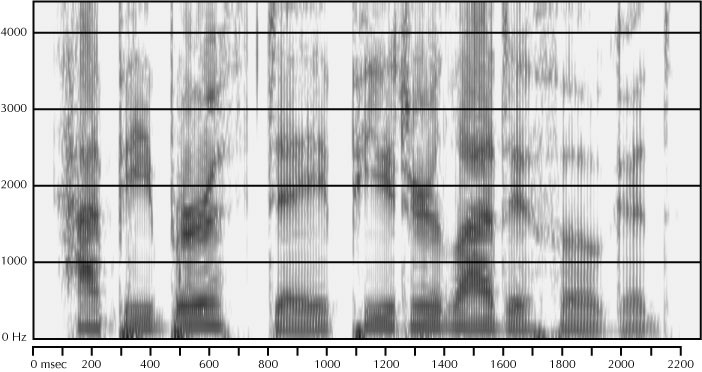
\includegraphics[width = \linewidth]{figs/Specrtogram.png}
    \end{multicols}
\end{frame}

\begin{frame}{Spectrograms}
    \begin{multicols}{2}
        \begin{itemize}
            \item Time is on the x-axis
            \item Component frequencies on the y-axis
            \item Shading shows amplitude, darker = higher amplitude
        \end{itemize}

        \columnbreak

        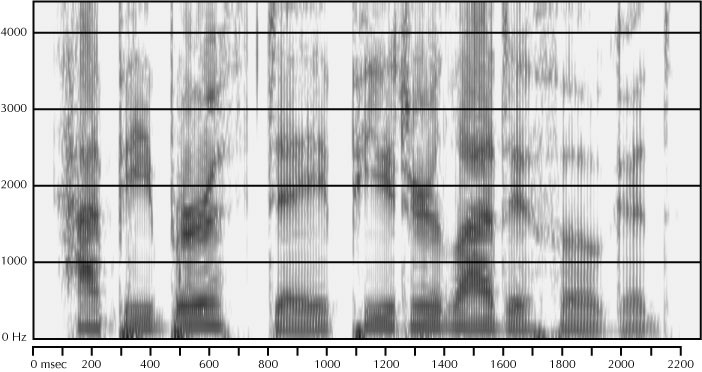
\includegraphics[width = \linewidth]{figs/Specrtogram.png}
    \end{multicols}
\end{frame}

\begin{frame}{Spectrogram}
    \begin{itemize}
        \item There’s a tradeoff between time and frequency in terms of resolution
        \item Two types of spectrograms
        \begin{itemize}
            \item Narrowband: shows frequency in more detail at the expense of changes over time
            \item Wideband: shows changes in time in more detail at the expense of frequency
        \end{itemize}
    \end{itemize}
\end{frame}

\begin{frame}{Frequency confusion}
    \begin{itemize}
        \item We need to be very specific about \textit{which} frequency we’re talking about because there are two references
        \begin{enumerate}
            \item The frequency of the complex wave we are analyzing
            \item The frequencies of the component parts
        \end{enumerate}
    \end{itemize}
\end{frame}

\begin{frame}{Fundamental frequency}
    \begin{itemize}
        \item The frequency of the complex wave we are decomposing is called the \textbf{fundamental} frequency, or $f0$
        \item In speech sounds, the rate of vocal fold vibration equals the fundamental
    \end{itemize}
\end{frame}

\begin{frame}{Harmonics}
    \begin{multicols}{2}
        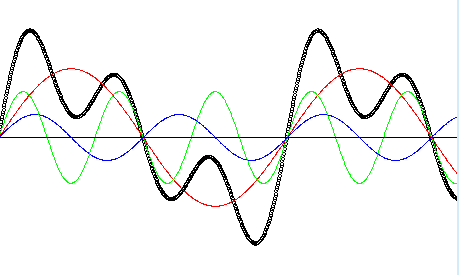
\includegraphics[width = \linewidth]{figs/Complex.png}

        \columnbreak

        \begin{itemize}
            \item The component parts of a complex wave each have their own frequencies
            \item These frequencies are called harmonics, because they are in a harmonic relationship with the fundamental
            \item Represented as $Hn$ where $n =$ a specific harmonic
        \end{itemize}
    \end{multicols}
\end{frame}

\begin{frame}{$f0$ and Harmonics}
    \begin{itemize}
        \item The harmonics are each an integer value of the fundamental
        \begin{itemize}
            \item $f0 = H1$ 
        \end{itemize}
        \item Meaning: a given harmonic, say the fourth one, is 4x the fundamental
        \item So, if the fundamental is 200Hz: 
        \begin{itemize}
            \item the first harmonic, H1 = 200Hz x 1 = ?Hz 
            \item the second harmonic, H2 = 200Hz x 2 = ?Hz 
            \item the third harmonic, H3 = 200Hz x 3 = ?Hz 
            \item the fourth harmonic, H4 = 200Hz x 4 = ?Hz 
            \item etc.
        \end{itemize}
    \end{itemize}
\end{frame}

\begin{frame}{$f0$ and Harmonics}
    \begin{itemize}
        \item The harmonics are each an integer value of the fundamental
        \begin{itemize}
            \item $f0 = H1$ 
        \end{itemize}
        \item Meaning: a given harmonic, say the fourth one, is 4x the fundamental
        \item So, if the fundamental is 200Hz: 
        \begin{itemize}
            \item the first harmonic, H1 = 200Hz x 1 = 200Hz 
            \item the second harmonic, H2 = 200Hz x 2 = 400Hz 
            \item the third harmonic, H3 = 200Hz x 3 = 600Hz 
            \item the fourth harmonic, H4 = 200Hz x 4 = 800Hz 
            \item etc.
        \end{itemize}
    \end{itemize}
\end{frame}

\begin{frame}{Where are the harmonics?}
    \begin{center}
        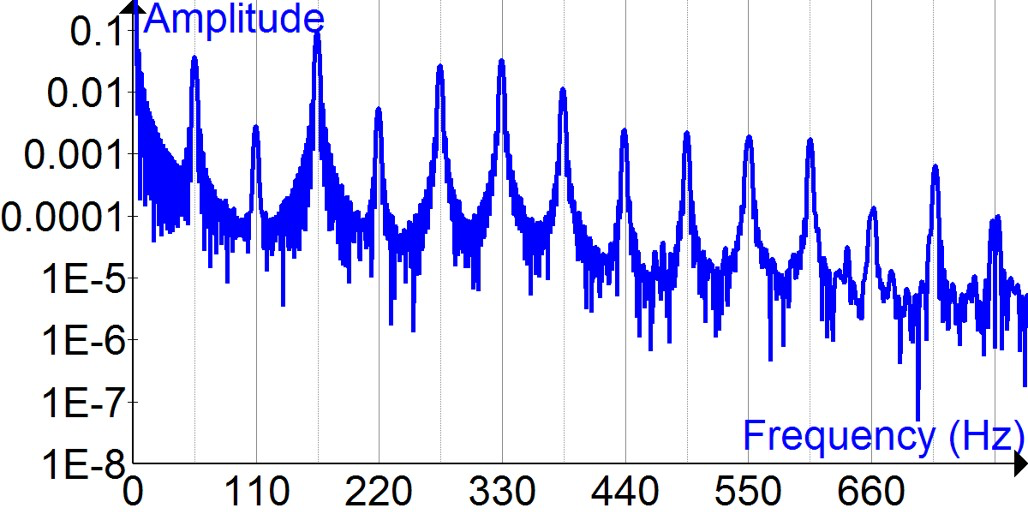
\includegraphics[width = 0.8\linewidth]{figs/Fourier-ComplexWaves.png}
    \end{center}
\end{frame}

\begin{frame}
    \frametitle{Playing with sound}
    \begin{center}
        {\Huge Playing around with Praat!}\\
        (if there is time)
    \end{center}
\end{frame}

%-----------------------------------------------------------
\section*{To Do:}
%-----------------------------------------------------------
\begin{frame}{To Do:}
    \begin{itemize}
        \item Complete the exit ticket for today on Canvas by 12:30pm.
        \item Submit your discussion posts on the readings
        \item Bring your computers for next time, we'll be playing with Praat and sound waves!!!
    \end{itemize}
\end{frame}

% \subsection<presentation>*{References}
% %-----------------------------------------------------------
% \begin{frame}[t,allowframebreaks]
%   \frametitle<presentation>{References}
%     \printbibliography
% \end{frame}

\end{document}